\documentclass[a4paper, 12pt]{article}
\usepackage[top=2.5cm, bottom=2.5cm, left=2.5cm, right=2.5cm]{geometry}
\usepackage[utf8]{inputenc}
\usepackage{amsmath, amsfonts, amssymb}
\usepackage[portuguese]{babel}
\usepackage{blkarray, bigstrut}
\usepackage{setspace}
\usepackage{graphicx}
\usepackage{amsmath}
\usepackage{tikz}
\usepackage{easybmat}

\begin{document}
 \begin{center}
  Curso de Tecnologia em Sistemas de Computação \\
  Disciplina : Banco de Dados \\
  AD1 - Primeiro Semestre de 2018 \\
  Professoras: Susana Makler e Sulamita Klein \\
  Nome: Fábio de Oliveira Branco\\ 
 \end{center}
 \begin{enumerate}
  \item \begin{enumerate}
  \item Falso, pois $\emptyset \subseteq \{\{\emptyset\}\}$. \\
  O correto seria afirmar que $\{\emptyset \} \in \{\{\emptyset\}\}$\\
  
  \item Falso, pois $\{\emptyset \} \in \{\{\emptyset\}\}$. \\
  O correto seria afirmar que $\{\{\emptyset\}\} \subseteq  \{\{\emptyset\}\}$
  \item Falso, podemos comprovar isso através do diagrama de Venn:\\ \\
  $A \cup (B - C)$:
  \begin{center}
    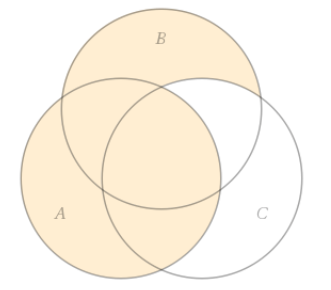
\includegraphics{img/primeiro.png}
  \end{center}
  $ (A - B) \cup (A - C)$:
  \begin{center}
    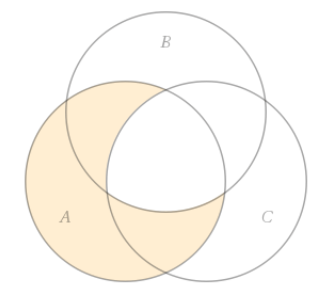
\includegraphics{img/segundo.png}
  \end{center}
  \end{enumerate}
  \newpage
 \end{enumerate}
\end{document}